\chapter{Introspective Analysis} \label{chapter:introspective}
%Introspective Analysis: Context-Sensitivity, Across the Board

\epigraph{The problem with introspection is that it has no end.}{\textit{Philip K. Dick}}

\emph{Points-to analysis} is probably the most common whole-program
static analysis, and often serves as a substrate for a variety of
high-level program analysis tasks. Points-to analysis computes the set
of objects (abstracted as their allocation sites) that a program
variable may point to during runtime. The promise, as well as the
challenge, of points-to analysis is to yield usefully precise
information without sacrificing scalability: the analysis inputs are
large and the analysis algorithms are typically quadratic or cubic,
but try to maintain near-linear behavior in practice, by exploiting
program properties and maintaining precision. Indeed precision and
performance often go hand-in-hand in a good points-to analysis
algorithm: better algorithms are often found to be both more precise
and faster, because smaller points-to sets lead to less work
\cite{1391987}.

\emph{Context-sensitivity} is a common way of pursuing precision and
scalability in points-to analysis. It consists of qualifying local
variables and objects with context information: the analysis unifies
information (e.g., ``what objects this method argument can point to'')
over all possible executions that map to the same context value, while
separating executions that map to different contexts. In this way,
context-sensitivity attempts to avoid precision loss from merging the
behavior of different dynamic program paths. Context-sensitivity comes
in many flavors, depending on the kind of context information, such as
\emph{call-site-sensitivity}
\cite{Sharir:Interprocedural,Shivers:1991:diss},
\emph{object-sensitivity}
\cite{Milanova:2002:POS:566172.566174,1044835}, and
\emph{type-sensitivity}~\cite{pointsto-popl11}.

An oft-remarked fact about context-sensitivity, however, is that even
the best algorithms have a common failure mode when they cannot
maintain precision. Past literature reports that ``the performance of
a [...]  deep-context analysis is bimodal'' \cite{pointsto-popl11};
``context-sensitive analyses have been associated with very large
numbers of contexts'' \cite{DBLP:conf/cc/LhotakH06}; ``algorithms
completely hit a wall after a few iterations, with the number of
tuples exploding
exponentially''~\cite{Liang:2011:SAR:1993498.1993567}.  Recent
published results~\cite{hybrid-pldi13} fail to run a
2-object-sensitive analysis in under 90mins for 2 of 10 DaCapo
benchmarks, while 2 more benchmarks take more than 1,000sec, although
most other benchmarks of similar or larger size get analyzed in under
200sec.

\begin{figure}[tbp]
\begin{center}
\hspace{-2mm}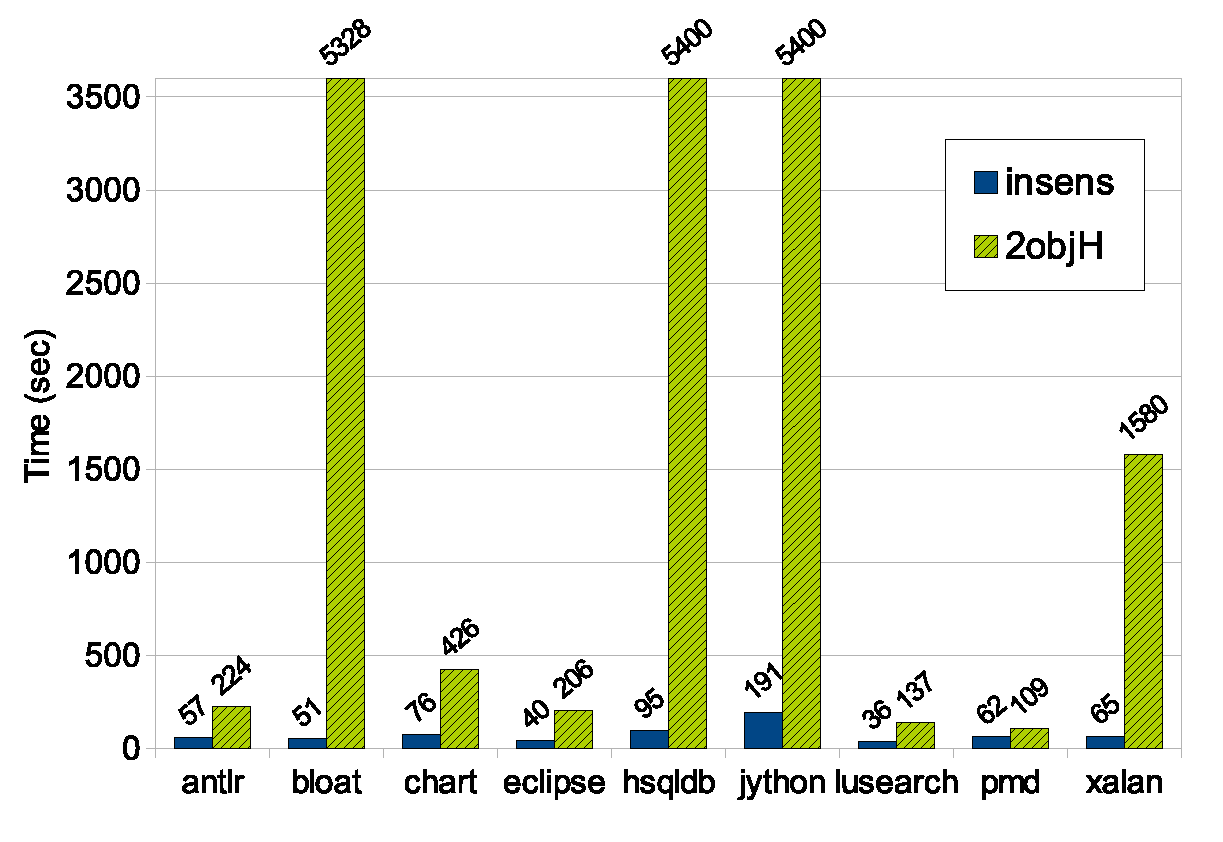
\includegraphics[scale=0.42]{assets/introspective/intro-chart.pdf}
\end{center}
\vspace{-0.6cm}
\caption{Comparison of running times of context-insensitive analysis vs.
  2-object-sensitive with context-sensitive heap. The y-axis is
  truncated to 1hr for readability.}
\label{intro-chart}
\end{figure}

Thus, when context-sensitivity works, it works formidably, in terms of
both precision and performance. When it fails, however, it fails
miserably, quickly exploding in complexity. In contrast,
context-insensitive analyses uniformly scale well, for the same
inputs. Figure~\ref{intro-chart} vividly demonstrates this phenomenon
for the DaCapo benchmarks, analyzed with the Doop
framework~\cite{BS-OOPSLA09} under a context-insensitive (insens)
analysis and a 2-object-sensitive analysis with a context-sensitive
heap (2objH). (The chart truncates the analysis time of the
longest-running benchmarks. Two of them, hsqldb and jython, timed out
after 90mins on a 24GB machine, and would not terminate even for much
longer timeouts.) As can be seen, context-insensitive analyses vary
relatively little in performance, while context-sensitivity often
causes running time (and memory use) to explode.

Faced with this unpredictability of context-sensitivity, a
common reaction is to avoid it, favoring context-insensitive analyses,
and, consequently, missing significant precision benefits for
well-behaved programs. Even worse, for some applications, eschewing
expensive context-sensitivity is not an option---a context-insensitive
analysis is just not good enough.
%, and even an often inexpensive
%context-sensitive analysis (e.g., 2-type-sensitive with a
%context-sensitive heap) fails to yield good precision. 
Reports from industry~\cite{cifuentes} and academic
researchers~\cite{chong} alike reiterate that precise
context-sensitivity is essential for information-flow analysis, taint analysis,
and other security analyses.

We can ask ourselves, why does this scalability barrier arise? The
core problem is that, for some objects or methods, the points-to
information is imprecise enough that more context does not help, while
incurring a heavy overhead \cite{pointsto-popl11}. Consider a method
argument that was found to point to $n$ objects by a less precise
analysis. Further analyzing the method in $c$ different contexts (or,
equivalently, increasing context depth by 1) will ideally yield $n/c$
points-to facts per context, perfectly splitting the previous
$n$-object points-to set.
%yielding both precision and scalability.
In the worst case, however, increasing the context depth will result
in $c$ copies of $n$ points-to facts each: the extra context depth
will not have yielded more precision, but will have multiplied the
space and time costs.
%When this occurs, the
%analysis cost explodes for greater context depths.

The focus of our work is on the detection and prevention of
pathological behavior in context-sensitive analyses, with minimal
intervention. In this way, we achieve many of the precision benefits
of context-sensitivity without sacrificing scalability. It does not
seem possible to know in advance (e.g., by identifying syntactic
features of the program) which program elements may be responsible for
pathological behavior. Nevertheless, we argue that it is possible to
identify such elements with a scalable context-insensitive analysis.
We introduce the concept of \emph{introspective context-sensitivity}:
during a first, context-insensitive, analysis pass, the analysis
observes symptoms indicating that the cost may get out of hand for
deeper context. This detects exactly the pathology identified
above. In its simplest form, the analysis will ask ``which program
sites currently have points-to information that may grow too large for
an extra level of context?''  Using a configurable second pass, such
sites will be re-analyzed with shallow context, even though the rest
of the program will be re-analyzed with a deeper context. Note that
this approach adaptively tunes the precision of the analysis for the
entire program, and not only for a single goal, as in earlier
\emph{refinement-based}~\cite{1134027} or
\emph{pruning}~\cite{Liang:2011:SAR:1993498.1993567} techniques---our
related work section includes a detailed discussion.

% The pattern
%can be repeated for more passes.

%This analysis runs first and informs the application of
%context-sensitivity---we use the term \emph{introspective
%  context-sensitive analysis} for the resulting approach. 

%As a
%general pattern, this approach is familiar.  Even in the context of
%points-to analysis, the pattern of performing a coarse-grained
%analysis and using it to tune a finer-grained one has been explored
%before---e.g., by Sridharan and Bod\'{\i}k~\cite{1134027} and by Liang
%and Naik~\cite{Liang:2011:SAR:1993498.1993567}. Nevertheless, such
%past approaches differ from our approach in terms of both external
%applicability and impact: they fundamentally apply to demand-driven
%(as opposed to all-points) analyses and they either do not target
%context depth or only apply to specific kinds of context---our related
%work section includes a detailed discussion.

%The key of our introspective approach is in exploring how exactly to
%use the outcome of a context-insensitive analysis to preemptively
%identify and eliminate sources of worst-case behavior for a
%context-sensitive analysis. 
%In intuitive terms, introspective
%context-sensitivity performs a cost-benefit calculation, with an
%emphasis on the potential cost of increasing context depth.
%, because cost can
%be estimated more reliably. 
%Fairly simple, yet not always obvious, heuristics 
%can estimate this cost well. 
%For instance, we can avoid refining methods at call
%sites that pass arguments with large points-to sets, avoid refining
%objects with both large points-to sets \emph{and} many variables
%pointing to them, etc.

%(i.e., analyzing
%context-sensitively) any methods with large cumulative sizes of
%points-to sets (over all the method's variables) or objects with large
%points-to sets in any of their fields. As we will see, such
%``obvious'' heuristics are strictly inferior to slightly more
%sophisticated ones that address the complexity explosion at its core.
%Sample good heuristics include ``determine whether to refine
%per-invocation-site and not per method'', ``avoid refining objects
%pointed to by many vars'', and more.

The net outcome of our work is not a ``first line of defense''
analysis, but an ``if all else fails'' analysis. Users are still
better advised to first use traditional context-sensitive algorithms,
in the hope that these will scale well and provide good
precision. When this fails, however, we show that we can provide a
highly reliable knob 
%for filtering out worst-case performance at a
%small cost in precision. Our experiments demonstrate 
so that the user can ``dial-in'' scalability, to the exact level
required. For instance, as seen in Figure~\ref{intro-chart}, a precise
2objH analysis fails to run in under 60mins on a 24GB machine for 3 of
our experimental subjects. However, we can get an introspective
context-sensitive analysis to scale to all benchmarks in under 12mins,
while still gaining significant precision over a context-insensitive
analysis. Yet another introspective analysis scales to all but one
benchmark in under 20mins, while sacrificing very little precision
(keeping about 2/3 of the precision gains of a full 2objH analysis).
%for most metrics
%This ability to tune the precision/scalability tradeoff
%is the main benefit that our approach offers.  
For call-site sensitive analyses, the gains are even more pronounced,
with several benchmarks exhibiting at least 300\% speedups.
% without sacrificing nearly any precision.

Overall, our paper makes the following contributions:

\begin{itemize}
\item We offer an approach to refining a context-sensitive analysis
  while avoiding its worst-case cost. The approach relies on first
  running a context-insensitive analysis and using its results to
  inform the application of context-sensitivity. Much of the challenge
  concerns the question of \emph{how} to use this information, i.e., 
  what heuristics yield good behavior.

\item We encode the approach in a simple form, by incremental modifications
  of a general declarative analysis pattern. Therefore, our approach
  works on virtually any algorithm expressed in this manner. Our
  implementation is on the Doop framework~\cite{BS-OOPSLA09} and already
  applies to the over 30 analysis algorithms that the framework has to offer.

\item We show experimentally the benefit of introspective
  context-sensitivity. We quantify the precision loss and scalability
  gains for different parameter settings and show that there is a dial
  that users can tune, to select points in this spectrum. Even our
  high-precision settings are effective in eliminating behavior outliers,
  showing that introspective context-sensitivity has core value:
  previously hopeless analyses suddenly become feasible, for little
  precision loss. We believe that the result is to give confidence
  that context-sensitive analyses can be used in virtually any setting
  and not just in the nebulous ``when they work well'' case.

\end{itemize}



\section{Formulation of Introspective Context-Sensitivity}
\label{model}

We demonstrate introspective context-sensitivity via incremental
changes to an existing model for context-sensitive,
flow-insensitive\footnote{\emph{Flow-sensitivity} refers to taking
  into account the intra-procedural control-flow of the
  program---e.g., that an instruction may always precede
  another. Flow-sensitivity can be approximated in a flow-insensitive
  setting by first putting the input in static-single-assignment (SSA)
  form.} points-to analysis
algorithms~\cite{exceptions-cc13,hybrid-pldi13}. The logical formalism
of this model is very close to the core components of our actual
analysis implementation. Therefore, the model acts both as background
and as a frame on which we will plug refinement logic in later
sections.

We model a multitude of points-to analyses together with online
call-graph construction as a parametric Datalog program.  Datalog
rules are monotonic logical inferences that repeatedly apply to infer
more facts until fixpoint. Our rules do not use negation in a
recursive cycle, or other non-monotonic logic constructs, resulting in
a declarative specification: the order of evaluation of rules or
examination of clauses cannot affect the final result. The same
abstract model applies to a wealth of analyses. We use it to model a
context-insensitive Andersen-style \cite{dvanhorn:andersen-phd94}
analysis, as well as several context-sensitive analyses:
call-site-sensitive \cite{Sharir:Interprocedural,Shivers:1991:diss},
object-sensitive~\cite{1044835}, and type-sensitive~\cite{pointsto-popl11}.

The input language is a representative simplified intermediate
language with a) a ``new'' instruction for allocating an object; b) a
``move'' instruction for copying between local variables; c) ``store''
and ``load'' instructions for writing to the heap (i.e., to object
fields); d) a ``virtual method call'' instruction that calls the
method of the appropriate signature defined in the dynamic
class of the receiver object. This language models well the Java
bytecode representation,\footnote{The Java bytecode language is a
  stack-based intermediate language, for reasons of compactness.  For
  analysis purposes, however, it is common to translate it into
  equivalent but more conventional notations, such as the Jimple
  intermediate language of the Soot
  framework~\cite{vall99soot,valleerai00optimizing}. It is more
  accurate to say that out intermediate language is a simplified form
  of Jimple, rather than a simplified form of the Java bytecode.} but
also other high-level intermediate languages. 
%(It does not, however,
%model languages such as C or C++ that can create pointers through an
%address-of operator. The techniques used in that space are fairly
%different---e.g., \cite{antgrasshopper,1480911}.) 
The specification of our points-to analysis as well as the input
language are in line with those in past literature
\cite{Guarnieri:2009:GMS:1855768.1855778,livshits12}, although we also
integrate elements such as on-the-fly call-graph construction and
field-sensitivity.

Specifying the analysis logically as Datalog rules has the advantage
that the specification is close to the actual implementation.  Datalog
has been the basis of several implementations of program analyses,
both low-level
\cite{repsdb,DBLP:conf/aplas/WhaleyACL05,1065169,996859,BS-OOPSLA09}
and high-level \cite{1368142,codequest}. Indeed, the analysis we show
is a faithful model of the implementation in the Doop
framework~\cite{BS-OOPSLA09}, upon which our work builds. Our
specification of the analysis
(Figures~\ref{fig:input}-\ref{fig:baserules}) is an abstraction of the
actual implementation in the following ways:

\begin{itemize}
\item The implementation has many more rules. It covers the full
  complexity of Java, including rules for handling reflection, native
  methods, static fields, string constants, implicit initialization,
  threads, and a lot more. The Doop
  implementation
%\footnote{Available at http://doop.program-analysis.org/} 
  contains over 600 rules in the common core of all analyses, and
  several more rules specific to each analysis, as opposed to the 10
  rules we examine here. (Note, however, that these few rules are the
  most crucial for points-to analysis. They also correspond fairly
  closely to the algorithms specified in other formalizations of
  points-to analyses in the
  literature~\cite{kcfa-pldi10,pointsto-popl11}.)

\item The implementation also reflects considerations for efficient
  execution. The most important is that of defining indexes for the
  key relations of the evaluation. Furthermore, it designates some
  relations as functions, defines storage models for relations (e.g.,
  how many bits each variable uses), designates intermediate relations
  as ``materialized views'' or not, etc. No such considerations are
  reflected in our model.
\end{itemize}



%\vspace{-5mm}
\begin{figure}[tb!p]
%\begin{center}
\hspace{-1mm}
\begin{tabular}{l}
%\begin{tabular}{llll}
%$V$ is a set of variables & $H$ is a set of heap abstractions \\
%$M$ is a set of methods & $S$ is a set of method signatures (including name) \\
%$F$ is a set of fields & $I$ is a set of instructions (e.g., invocation sites)\\
%$T$ is a set of class types & $\mathbb{N}$ is the set of natural numbers \\
%$HC$ is a set of heap contexts & $C$ is a set of contexts \\
%\end{tabular}
\small $V$ is a set of program variables \\
\small $H$ is a set of heap abstractions (i.e., allocation sites) \\
\small $M$ is a set of method identifiers \\
\small $S$ is a set of method signatures (including name, type signature) \\
\small $F$ is a set of fields \\
\small $I$ is a set of instructions (mainly used for invocation sites)\\
\small $T$ is a set of class types \\
\small $\mathbb{N}$ is the set of natural numbers \\
\small $C$ is a set of (calling) contexts \\
\small $HC$ is a set of heap contexts \\
%\\
\cline{1-1}
\hspace{-3mm}
\begin{tabular}{l l}
\pred{Alloc}{var : V, heap : H, inMeth : M}  & \args{\# var = new ...} \\
\pred{Move}{to : V, from : V}                & \args{\# to = from} \\
\pred{Load}{to : V, base : V, fld : F}       & \args{\# to = base.fld}\\
\pred{Store}{base : V, fld : F, from : V}    & \args{\# base.fld = from} \\
\pred{VCall}{base : V, sig : S, invo : I, inMeth : M} & \args{\# base.sig(..)}   \\
\end{tabular}\\
\\
\pred{FormalArg}{meth : M, i : $\mathbb{N}$, arg : V} \\ 
\pred{ActualArg}{invo : I, i : $\mathbb{N}$, arg : V} \\ 
\pred{FormalReturn}{meth : M, ret : V} \\                
\pred{ActualReturn}{invo : I, var : V} \\                
\pred{ThisVar}{meth : M, this : V} \\                    
\pred{HeapType}{heap : H, type : T} \\
\pred{LookUp}{type : T, sig : S, meth : M} \\            
\\
\pred{SiteToRefine}{invo : I, meth : M} \\ 
\pred{ObjectToRefine}{heap : H} \\ 
\cline{1-1}
\pred{VarPointsTo}{var : V, ctx : C, heap : H, hctx : HC} \\
\pred{CallGraph}{invo : I, callerCtx : C, meth : M, calleeCtx : C} \\
\pred{FldPointsTo}{baseH: H, baseHCtx: HC, fld: F, heap: H, hctx: HC} \\
\pred{InterProcAssign}{to : V, toCtx : C, from : V, fromCtx : C} \\
\pred{Reachable}{meth : M, ctx : C} \\
%\\
\cline{1-1}
\cons{Record}{heap : H, ctx : C}{newHCtx : HC} \\
\cons{Merge}{heap : H, hctx : HC, invo : I, ctx : C}{newCtx : C} \\
\cons{RecordRefined}{heap : H, ctx : C}{newHCtx : HC} \\
\cons{MergeRefined}{heap : H, hctx : HC, invo : I, ctx : C}{newCtx : C} \\
%\\
%\cline{1-1}
\end{tabular}
%\end{center}
\caption[]{Our domain, input relations, output relations, and
  constructors of contexts. The input relations are of three kinds:
  relations encoding program instructions (the kind of instruction is
  shown in a comment), relations encoding type system and other
  environment information, and relations that filter which
  call-sites/target methods and which objects should have a different
  (i.e., more precise) context in introspective context-sensitivity.}
%\caption[]{Our domain, input relations (representing program instructions---with
%the matching program pattern shown in a comment---and type
%information), output relations, and constructors of contexts.}
\label{fig:input}
\end{figure}


\begin{figure}[tb!p]
%\begin{center}
\begin{tabular}{l}
%\cline{1-1}
\pred{InterProcAssign}{to, calleeCtx, from, callerCtx} \rulearrow{} \\
\hspace{2 mm} \pred{CallGraph}{invo, callerCtx, meth, calleeCtx}, \\
\hspace{2 mm} \pred{FormalArg}{meth, i, to}, \pred{ActualArg}{invo, i, from}. \\
\\

\pred{InterProcAssign}{to, callerCtx, from, calleeCtx} \rulearrow{} \\
\hspace{2 mm} \pred{CallGraph}{invo, callerCtx, meth, calleeCtx}, \\
\hspace{2 mm} \pred{FormalReturn}{meth, from}, \pred{ActualReturn}{invo, to}. \\
\\
\\
\cons{Record}{heap, ctx}{hctx}, \\
\pred{VarPointsTo}{var, ctx, heap, hctx} \rulearrow{} \\
\hspace{2 mm} \pred{Reachable}{meth, ctx}, \pred{Alloc}{var, heap, meth}, \\
\hspace{2 mm} !\pred{ObjectToRefine}{heap}. \\
\\

\args{\# duplicate rule, for introspective context-sensitivity}\\
\cons{RecordRefined}{heap, ctx}{hctx}, \\
\pred{VarPointsTo}{var, ctx, heap, hctx} \rulearrow{} \\
\hspace{2 mm} \pred{Reachable}{meth, ctx}, \pred{Alloc}{var, heap, meth}, \\
\hspace{2 mm} \pred{ObjectToRefine}{heap}. \\
\\

\pred{VarPointsTo}{to, ctx, heap, hctx} \rulearrow{} \\
\hspace{2 mm} \pred{Move}{to, from}, \pred{VarPointsTo}{from, ctx, heap, hctx}. \\
\\

\pred{VarPointsTo}{to, toCtx, heap, hctx} \rulearrow{} \\
\hspace{2 mm} \pred{InterProcAssign}{to, toCtx, from, fromCtx}, \\
\hspace{2 mm} \pred{VarPointsTo}{from, fromCtx, heap, hctx}. \\
\\

\pred{VarPointsTo}{to, ctx, heap, hctx} \rulearrow{} \\
\hspace{2 mm} \pred{Load}{to, base, fld}, \pred{VarPointsTo}{base, ctx, baseH, baseHCtx}, \\
\hspace{2 mm} \pred{FldPointsTo}{baseH, baseHCtx, fld, heap, hctx}. \\
\\

\pred{FldPointsTo}{baseH, baseHCtx, fld, heap, hctx} \rulearrow{} \\
\hspace{2 mm} \pred{Store}{base, fld, from}, \pred{VarPointsTo}{from, ctx, heap, hctx},\\
\hspace{2 mm} \pred{VarPointsTo}{base, ctx, baseH, baseHCtx}. \\
\\
\\
\cons{Merge}{heap, hctx, invo, callerCtx}{calleeCtx}, \\
\pred{Reachable}{toMeth, calleeCtx}, \\
\pred{VarPointsTo}{this, calleeCtx, heap, hctx}, \\
\pred{CallGraph}{invo, callerCtx, toMeth, calleeCtx} \rulearrow{} \\
\hspace{2 mm} \pred{VCall}{base, sig, invo, inMeth}, \pred{Reachable}{inMeth, callerCtx}, \\
\hspace{2 mm} \pred{VarPointsTo}{base, callerCtx, heap, hctx},\\
\hspace{2 mm} \pred{HeapType}{heap, heapT}, \pred{Lookup}{heapT, sig, toMeth},\\
\hspace{2 mm} \pred{ThisVar}{toMeth, this}, \\
\hspace{2 mm} !\pred{SiteToRefine}{invo, toMeth}. \\

\\
\args{\# duplicate rule, for introspective context-sensitivity}\\
\cons{MergeRefined}{heap, hctx, invo, callerCtx}{calleeCtx}, \\
\pred{Reachable}{toMeth, calleeCtx}, \\
\pred{VarPointsTo}{this, calleeCtx, heap, hctx}, \\
\pred{CallGraph}{invo, callerCtx, toMeth, calleeCtx} \rulearrow{} \\
\hspace{2 mm} \pred{VCall}{base, sig, invo, inMeth}, \pred{Reachable}{inMeth, callerCtx}, \\
\hspace{2 mm} \pred{VarPointsTo}{base, callerCtx, heap, hctx},\\
\hspace{2 mm} \pred{HeapType}{heap, heapT}, \pred{Lookup}{heapT, sig, toMeth},\\
\hspace{2 mm} \pred{ThisVar}{toMeth, this}, \\
\hspace{2 mm} \emph{\pred{SiteToRefine}{invo, toMeth}}. \\
 \\
%\cline{1-1}
\end{tabular}
%\end{center}
\caption[]{Datalog rules for the points-to analysis and call-graph construction.}
\label{fig:baserules}
\end{figure}

Figure~\ref{fig:input} shows the domain of our analysis (i.e., the
different value sets that constitute the space of our computation),
its input relations, the intermediate and output relations, as well as
four constructor functions, responsible for producing new
contexts. Figure~\ref{fig:baserules} shows the points-to analysis and
call-graph computation. 

\paragraph{Input relations.}
  The input relations correspond to the intermediate language for our
  analysis. They are logically grouped into relations that represent
  instructions, relations that represent name-and-type information,
  and parameterization relations for introspective
  context-sensitivity. For instance, the \predname{Alloc} relation
  represents every instruction that allocates a new heap object,
  \args{heap}, and assigns it to local variable \args{var} inside
  method \args{inMeth}. (Note that every local variable is defined in
  a unique method, hence the \args{inMeth} argument is also implied by
  \args{var} but is included to simplify later rules.) There are
  similar input relations for all other instruction types
  (\predname{Move}, \predname{Load}, \predname{Store}, and
  \predname{VCall}).

  Similarly, there are relations that encode type system, symbol
  table, and program environment information. These are mostly
  straightforward. For instance, \predname{FormalArg} shows which
  variable is a formal argument of a given method at a certain index
  (i.e., the $i$-th argument). \predname{LookUp} matches a method
  signature to the actual method definition inside a
  type. \predname{HeapType} matches an object to its type, i.e., is a
  function of its first argument. (Note that we are shortening the
  term ``heap object'' to just ``heap'' and represent heap objects as
  allocation sites throughout.) \predname{ActualReturn} is also a
  function of its first argument (a method invocation site) and
  returns the local variable at the call-site that receives the method
  call's return value. 

  Finally, the \predname{SiteToRefine} and \predname{ObjectToRefine}
  relations are inputs that are used exclusively for the purposes of
  introspective context-sensitivity. They encode the program points
  (allocation sites, \args{heap}, and invocation site/method
  combinations, \args{invo}, \args{meth}) that will employ a different
  context abstraction from the rest.
  
\paragraph{Computed relations.}
  There are five output or intermediate computed relations:
  \predname{VarPointsTo}, $\ldots$,
  \predname{Reachable}.\footnote{\predname{Reachable} is somewhat of a
    special case, since we assume it is also used as an input
    relation: it needs to initially hold methods that are always
    reachable, such as the programs's \code{main} method, the
    constructor of class \code{java.lang.ClassLoader}, and more.  We
    ignore this technicality in the model, rather than burden our
    rules with a separate input relation.}  Every occurrence of a
  method or local variable in computed relations is qualified with a
  context (i.e., an element of set \args{C}), while every occurrence
  of a heap object is qualified with a heap context (i.e., an element
  of \args{HC}). The main output relations are \predname{VarPointsTo}
  and \predname{CallGraph}, encoding our points-to and call-graph
  results. The \predname{VarPointsTo} relation links a variable
  (\args{var}) to a heap object (\args{heap}). Other intermediate
  relations (\predname{FldPointsTo}, \predname{InterProcAssign},
  \predname{Reachable}) correspond to standard concepts and are
  introduced for conciseness and readability.

\paragraph{Constructors for context-sensitivity.}
  The base rules are not concerned with what kind of
  context-sensitivity is used. The same rules can be used for a
  context-insensitive analysis (by only ever creating a single context
  object), for a call-site-sensitive analysis, or for an
  object-sensitive analysis, for any context depth. These aspects are
  completely hidden behind constructor functions \consname{Record} and
  \consname{Merge}, and their counterparts \consname{RecordRefined}
  and \consname{MergeRefined}, used for introspective
  context-sensitivity---as explained below.  \consname{Record} and
  \consname{Merge} follow the usage and naming convention of earlier
  work~\cite{pointsto-popl11,hybrid-pldi13}. \consname{Record} takes
  all available information at the allocation site of an object and
  combines it to produce a new heap context, while \consname{Merge}
  takes all available information at the call site of a method and
  combines it to create a new calling context (or just ``context'').
  Heap contexts qualify heap objects in order to provide more
  fine-grained differentiation than mere allocation sites.  Calling
  contexts are used to qualify method calls, i.e., they are used for
  local variables in a program. In this way, variables that pertain to
  different invocations of the same method are distinguished, as much
  as the context granularity allows.  These functions are sufficient
  for modeling a very large variety of context-sensitive
  analyses. Explaining the different kinds of context-sensitivity
  produced by varying \consname{Record} and \consname{Merge} is beyond
  the scope of this paper---this approach is inherited from past
  literature\cite{pointsto-popl11, hybrid-pldi13}.  To give a single
  example, however, a 1-call-site-sensitive analysis with a
  context-sensitive heap has $C = HC = I$ (i.e., both the context and
  the heap context are a single instruction), \cons{Record}{heap,
    ctx}{ctx} and \cons{Merge}{heap, hctx, invo,
    callerCtx}{invo}. That is, when a method is called, its context is
  its call-site (\args{invo}) and when an object is allocated, its
  heap context is the context (\args{ctx}) of the allocating method
  (i.e., the call-site that invoked the allocating method).

  The \consname{RecordRefined} and \consname{MergeRefined}
  constructors are directly analogous to \consname{Record} and
  \consname{Merge} but just apply to different program points. These
  constructors are the machinery for introspective
  context-sensitivity: they vary the context-sensitivity of the
  analysis for a subset of the heap objects and methods.


\paragraph{Analysis logic.}
  The rule syntax in Figure~\ref{fig:baserules} is simple: the
  left arrow symbol (\rulearrow) separates the inferred facts (i.e.,
  the \emph{head} of the rule) from the previously established facts
  (i.e., the \emph{body} of the rule). For instance, the first rule
  states that, if we have computed a call-graph edge between
  invocation site \args{invo} and method \args{meth} (under some
  contexts), then we infer an inter-procedural assignment to the
  $i$-th formal argument of \args{meth} from the $i$-th actual
  argument at \args{invo}, for every $i$.

  The last rule (in duplicate) is the most involved. It states that if
  the original program has an instruction making a virtual method call
  over local variable \args{base} (this is an input fact), and the
  computation so far has established that \args{base} can point to
  heap object \args{heap} under a context for which the method is
  reachable, then the called method is looked up by-signature inside
  the type of \args{heap} and several further facts are inferred: that
  the looked up method is reachable, that it has an edge in the
  call-graph from the current invocation site, and that its
  \args{this} variable can point to \args{heap}. Additionally, the
  \consname{Merge}/\consname{MergeRefined} function is used to possibly
  create (or look up) the right context for the current invocation.

  Note that the rules that use context constructors (\consname{Record}
  and \consname{Merge}) are essentially duplicated. (In the full
  implementation, there are some two-dozen rules that construct new
  contexts, instead of the two in the model, and all are duplicated
  accordingly.) Each rule has two versions: one for objects
  (resp. method calls) that should have a default context and one for
  those that should have a different, refined context. Therefore, we
  can effect any change we want to the context-sensitivity of an
  analysis, on a per-object/per-site basis, by supplying the right
  input relations \predname{ObjectToRefine} or \predname{SiteToRefine}
  and setting the appropriate constructors, \consname{RecordRefined}
  and \consname{MergeRefined} to implement a different flavor of
  context-sensitivity. We discuss such options next.


\section{How To Selectively Refine}
\label{heuristics}

The model of the previous section allows configurability of
context-sensitivity in a large variety of ways. For instance, some
methods (or some call-sites) can be analyzed with object-sensitivity
while others are analyzed with call-site sensitivity, of any
depth. One aspect to determine, therefore, is the two analyses that
will be used in different program points.

Another question is how to populate the \predname{ObjectToRefine} and
\predname{SiteToRefine} input relations.  One could attempt to do so
by mere syntactic inspection of the program.  For example, methods
containing cast statements can be analyzed with a higher context
depth. In our work, we have failed to identify such syntactic
heuristics that would yield benefit.

Instead, our introspective context-sensitivity consists of running the
analysis \emph{twice}. The first time, \predname{ObjectToRefine} and
\predname{SiteToRefine} are empty and the
\consname{Merge}/\consname{Record} context constructors are set so
that an inexpensive but scalable analysis is performed. In our
experimental setting, these constuctor functions return a unique
constant value, \args{$\star$}, resulting in a context-insensitive
analysis:
\begin{quote}
\cons{Record}{heap,ctx}{$\star$}\\
\cons{Merge}{heap, hctx, invo, ctx}{$\star$} \\
\end{quote}

The \consname{MergeRefined} and \consname{RecordRefined} constructors
are set to implement an expensive context-sensitive analysis,
following the techniques of Kastrinis and
Smaragdakis~\cite{hybrid-pldi13}.  Yet, these constructors are not
relevant in the first analysis run, since the rules employing them are
predicated on having elements in \predname{SiteToRefine} and
\predname{ObjectToRefine}, respectively.

Subsequently, we use the results of the context-insensitive analysis
to compute which program elements to refine (i.e., to populate the
\predname{SiteToRefine} and \predname{ObjectToRefine} relations), and
run the analysis a second time. The result is that a subset of the
program elements are analyzed context-sensitively, while the rest are
analyzed context-insensitively even during the second analysis run.
In practical terms, the former set is larger than the latter: we focus
on identifying a relatively small number of program elements that may
disproportionately affect analysis costs and to analyze them
context-insensitively, while the majority of program elements are
analyzed context-sensitively.

Therefore, the main challenge is to identify a program query/client
analysis (over the results of a context-insensitive points-to
analysis) to predict which program elements should not be refined. Our
criterion is based on cost rather than expected benefit, since the
latter is very hard to estimate in an all-points (as opposed to
demand-driven) program analysis. There are several cost metrics that
we can mix-and-match to create introspective analysis heuristics.

\begin{enumerate}
\item \label{metric-arginflow} Compute at every invocation site the cumulative
  size of all points-to sets of actual arguments to the method call.
  (This is the argument \emph{in-flow} of the method call.)

\item \label{metric-methvpt} Compute for every method the cumulative
  (or maximum, for a variant of the metric) size of points-to sets
  over all local variables. (This is the method's \emph{total points-to volume}
  or \emph{max var-points-to}.)

\item \label{metric-maxfield} Compute for each object (i.e.,
  allocation site) the maximum (or total, for a variant of the metric)
  field points-to set over all of its fields (This is the object's \emph{max field points-to}, 
  or \emph{total field points-to}.)

\item \label{metric-methodmaxfield} Compute for every method the 
  maximum max field-points-to (metric~\ref{metric-maxfield}) among objects pointed to
  by the method's local variables. (This is the method's \emph{max var-field points-to}.)

\item \label{metric-pointedby} Compute for each object (i.e., allocation site) the
  number of local variables pointing to it. (This is the object's \emph{pointed-by} metric.)
\end{enumerate}

As can be seen, these metrics can vary in sophistication but all of
them attempt to estimate the cost that will be incurred if the same
method or allocation site were to be analyzed
context-sensitively. Indeed, our emphasis is not on the sophistication
of the metrics or on their fine-tuning. Instead, it is on their
simplicity and ease of composition so that one can create
parameterizable analyses: a knob for adjusting the
precision/scalability tradeoff. For example, we propose two heuristic
combinations of these metrics:

\begin{itemize}
% tempH heuristic in the initial source code
\item \emph{Heuristic A}: Refine all allocation sites except those
  with a \emph{pointed-by} (metric~\#\ref{metric-pointedby}) higher than
  a constant $K$.  Refine all method call sites except those with
  either an \emph{in-flow} (metric~\#\ref{metric-arginflow}) higher than
  a constant $L$ or a \emph{max var-field points-to}
  (metric~\#\ref{metric-methodmaxfield}) higher than a constant $M$.

% tempO heuristic in the initial source code
\item \emph{Heuristic B}: Refine all method calls sites except those
  that invoke methods with a \emph{total points-to volume}
  (metric~\#\ref{metric-methvpt}) above a constant $P$. Refine all
  object allocations except those for which the product of \emph{total
    field points-to} and \emph{pointed-by} (metrics
  \#\ref{metric-maxfield} and \#\ref{metric-pointedby}) exceeds a
  constant $Q$. The product of these two metrics can be seen as an
  object's total potential for weighing down the analysis.
\end{itemize}

These heuristics are themselves tunable, by adjusting the constant
parameters.  In the rest of the paper, when we refer to
\emph{Heuristic A} in measurements, the values of $K$, $L$, $M$ will
be 100, 100, and 200, respectively; when we refer to \emph{Heuristic
  B}, the values of $P$ and $Q$ will both be 10000. The point of
picking clear-cut reference numbers is to argue that the value of the
technique does not come from excessive tuning but from the underlying
power of the introspective analysis idea---even relatively large variations of
these numbers make scarcely any difference in the total picture of
results over multiple programs.

\paragraph{Discussion: Intuition.} 
The main insight behind our heuristic approach is that there are many
program elements whose analysis cost is vastly disproportionate to
their importance. If such elements are analyzed less precisely, the
analysis will avoid significant burden without incurring large
precision losses. The above two heuristics try to estimate
``disproportionate cost'' but have no way of estimating the
``importance'' of a program element. It would be an interesting
direction for future work to estimate this importance, i.e., to define
metrics that capture the extent of the impact of a program element's
precision on all other program elements.


%Furthermore, a program element with very large cost, in terms of associated
%points-to facts, may be hopeless for good enough precision anyway.
%On the other hand, the above intuition could potentially backfire:
%it is possible that context-sensitivity can productively distinguish
%seemingly-imprecise program elements (e.g., methods with large
%cumulative points-to sets, but also many callers) and maintain precision.


\paragraph{Implementation.}
The above metrics and heuristics can be easily implemented as short
analyses over the result of a context-insensitive points-to
analysis. For instance, the implementation of the \emph{in-flow}
metric (\#\ref{metric-arginflow}) is the following Datalog query,
which defines an intermediate predicate and aggregates over it.
(``\_'' is a nameless variable denoting any value, and
\emph{agg$<$...$>$} denotes an aggregation operation---in this case a
total count of matching tuples.)

\begin{figure}[h]
\begin{tabular}{l}
\pred{HeapsPerInvocationPerArg}{invo, arg, heap} \rulearrow{} \\
\hspace{2 mm} \pred{CallGraph}{invo, \_, \_, \_},\\
\hspace{2 mm} \pred{ActualArg}{invo, \_, arg},\\
\hspace{2 mm} \pred{VarPointsTo}{arg, \_, heap, \_}.\\
\\
\pred{InFlow}{invo, result} \rulearrow{} \\
\hspace{2 mm} \emph{agg}$<$\args{result = count()}$>$\\
\hspace{2 mm} (\pred{HeapsPerInvocationPerArg}{invo, \_, \_}).\\
\end{tabular}
\end{figure}

\vspace{-2mm}
\noindent Our implementation, including the appropriate modifications
of the Doop framework to implement the model of Section~\ref{model},
is open source and available at: $<$anonymized$>$.


\section{Evaluation}

Our evaluation setting uses the LogicBlox Datalog engine, v.3.9.0, on
a Xeon E5530 2.4GHz machine with only one thread running at a time and
24GB of RAM. We analyze the DaCapo benchmark programs (v.2006-10-MR2)
with Open JDK 1.6.0\_24. We run all benchmarks with default Doop
settings, including full reflection support.
%precision enabled, unlike prior
%published work \cite{pointsto-popl11,lhotak-callgraph12} which
%disables reflection for jython and hsqldb. 
We selected a priori 6 of the Dacapo benchmarks as our experimental
subjects: these are the programs that exhibit scalability problems
based on past literature~\cite{hybrid-pldi13} (confirmed by our own
experiments). Other benchmarks typically run in half the time of the
fastest benchmark of our set for deep context-sensitive analyses.
%% This is disproved for antlr in Figure 1.
% for a 2objH analysis.
Since our technique is explicitly not a ``first line of defense'',
benchmarks that are already certain to scale are out of scope.


\begin{figure*}[tbp]
\begin{center}
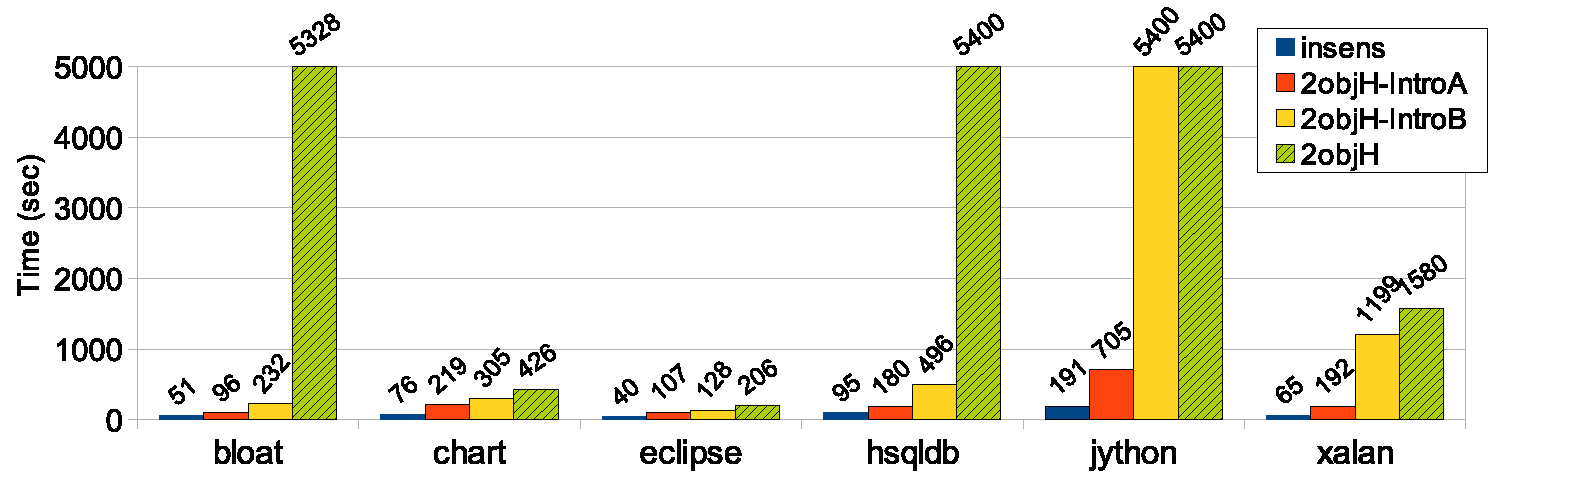
\includegraphics[scale=0.54]{assets/introspective/2objHtime.pdf} \\
%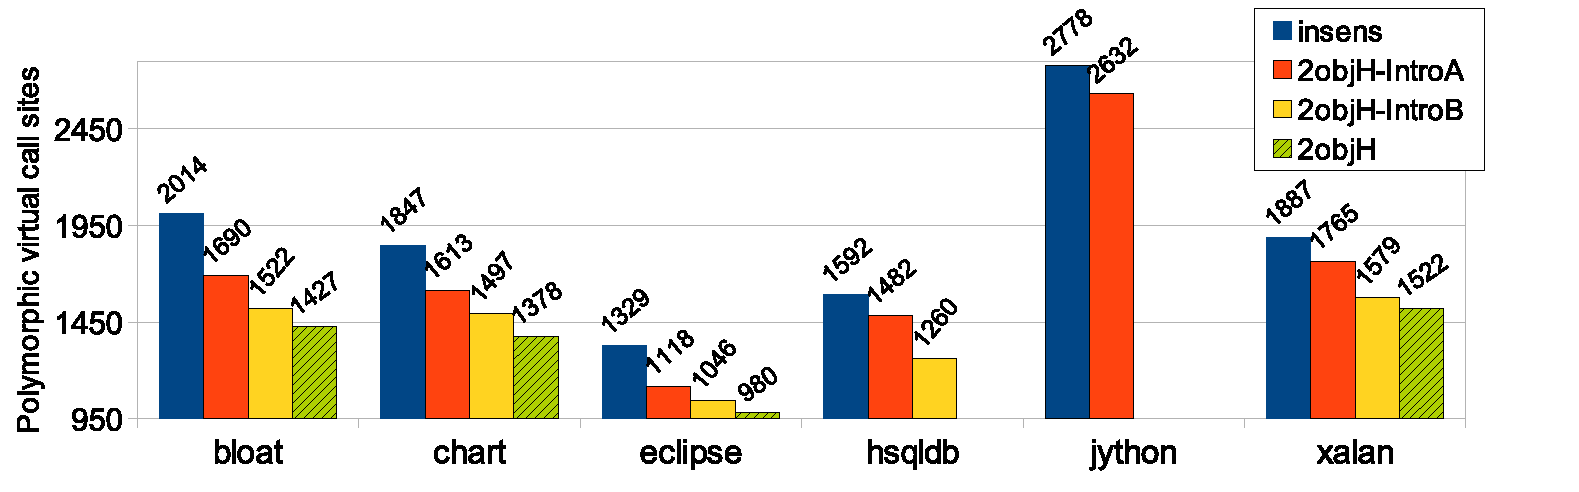
\includegraphics[width=16cm, height=4.6cm]{assets/introspective/2objHvcalls.pdf} \\
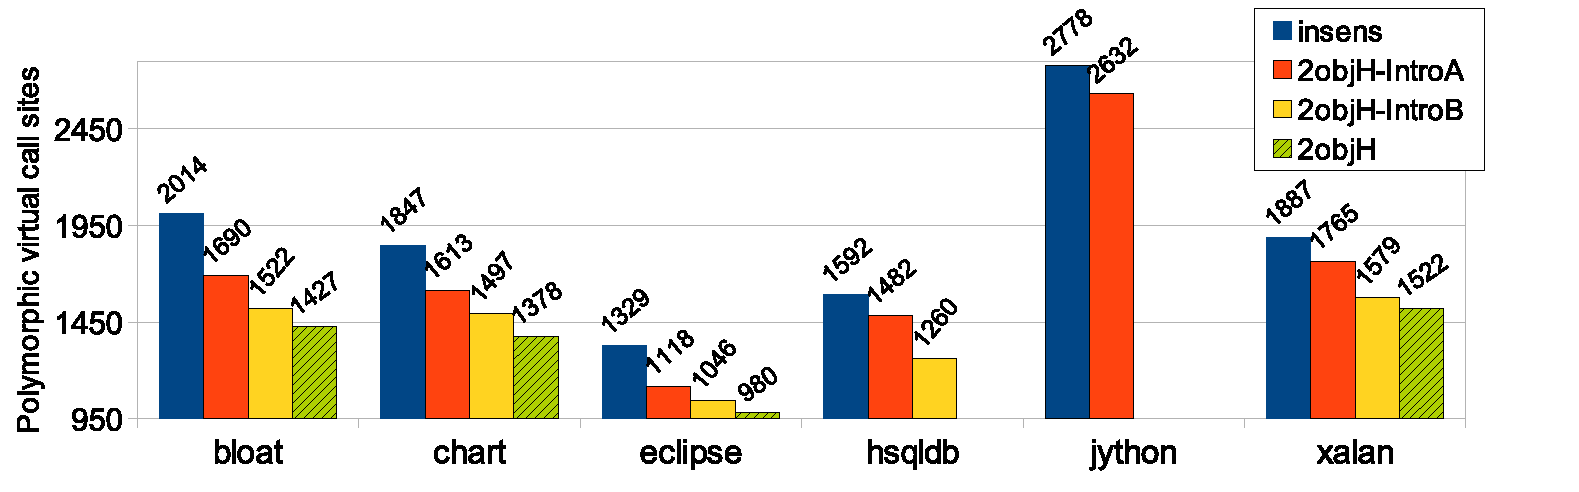
\includegraphics[scale=0.54]{assets/introspective/2objHvcalls.pdf} \\
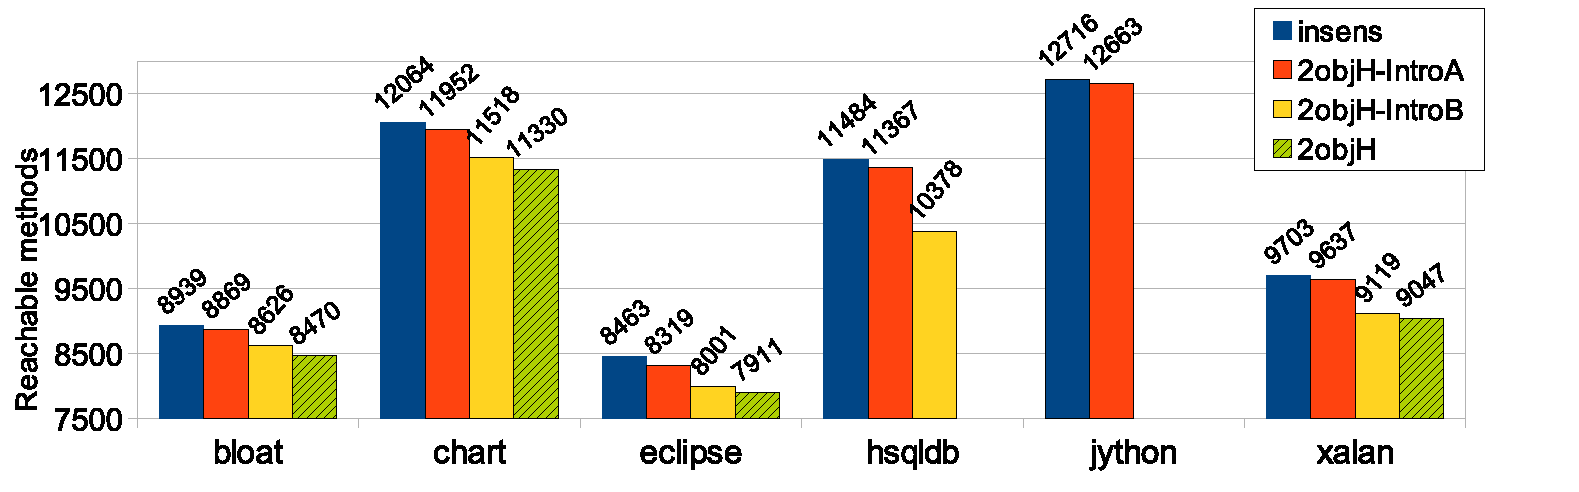
\includegraphics[scale=0.54]{assets/introspective/2objHmeths.pdf} \\
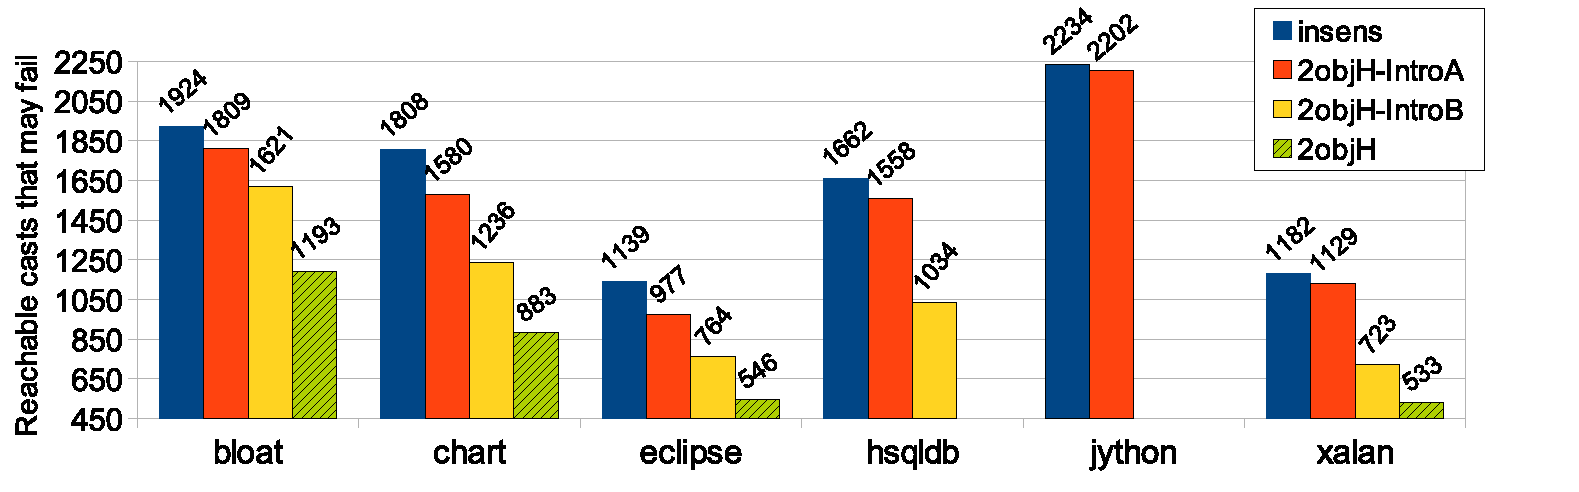
\includegraphics[scale=0.54]{assets/introspective/2objHcasts.pdf}
\end{center}
\vspace{-0.65cm}
\caption{Performance and precision (3 separate metrics: calls that
  cannot be devirtualized, reachable methods, casts that cannot be
  eliminated) for introspective context-sensitive variants of a 2objH
  analysis, compared with baselines (2objH and insensitive).}
\label{2objH-chart}
\end{figure*}


\begin{figure*}[tbp]
\begin{center}
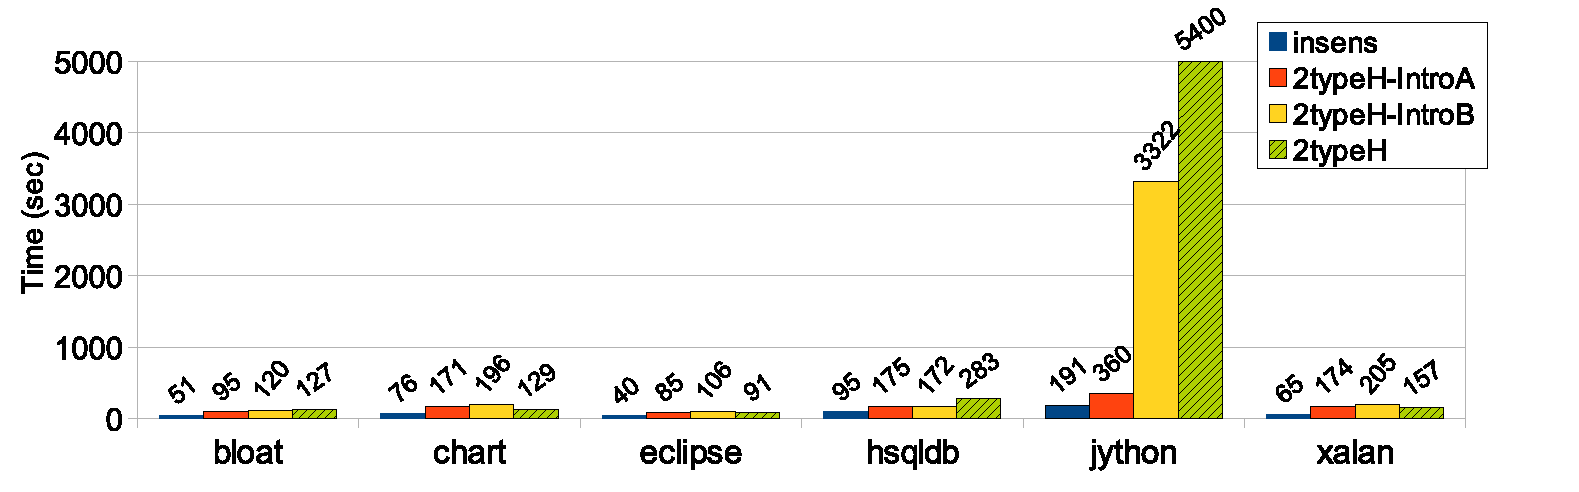
\includegraphics[scale=0.54]{assets/introspective/2typeHtime.pdf} \\
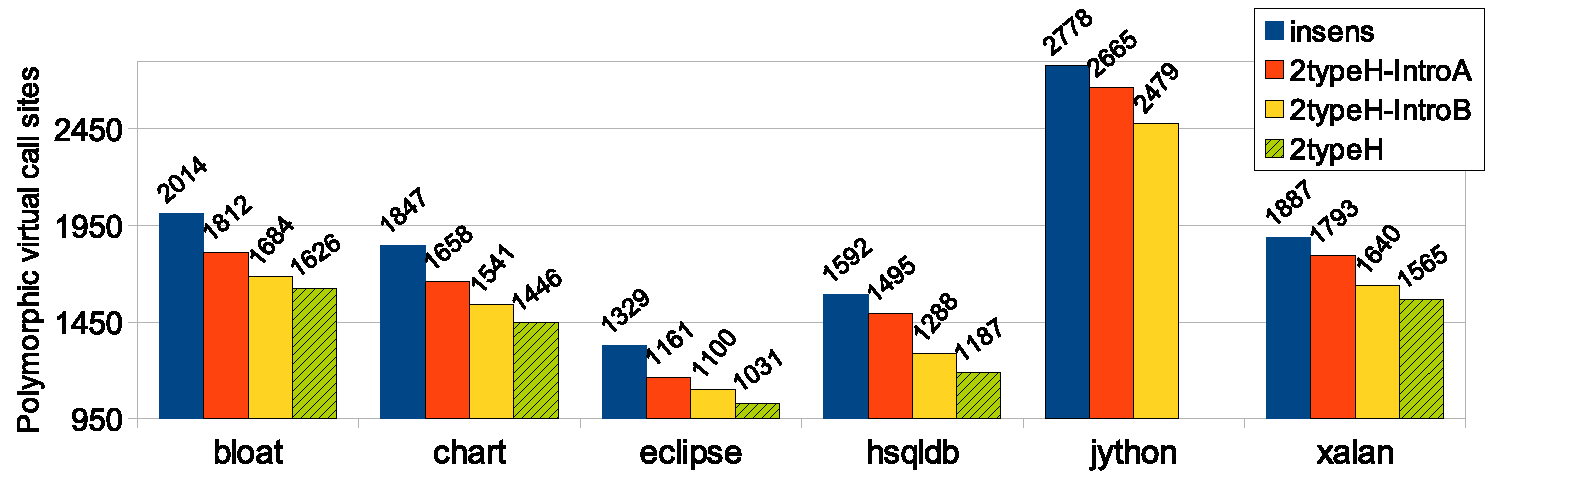
\includegraphics[scale=0.54]{assets/introspective/2typeHvcalls.pdf} \\
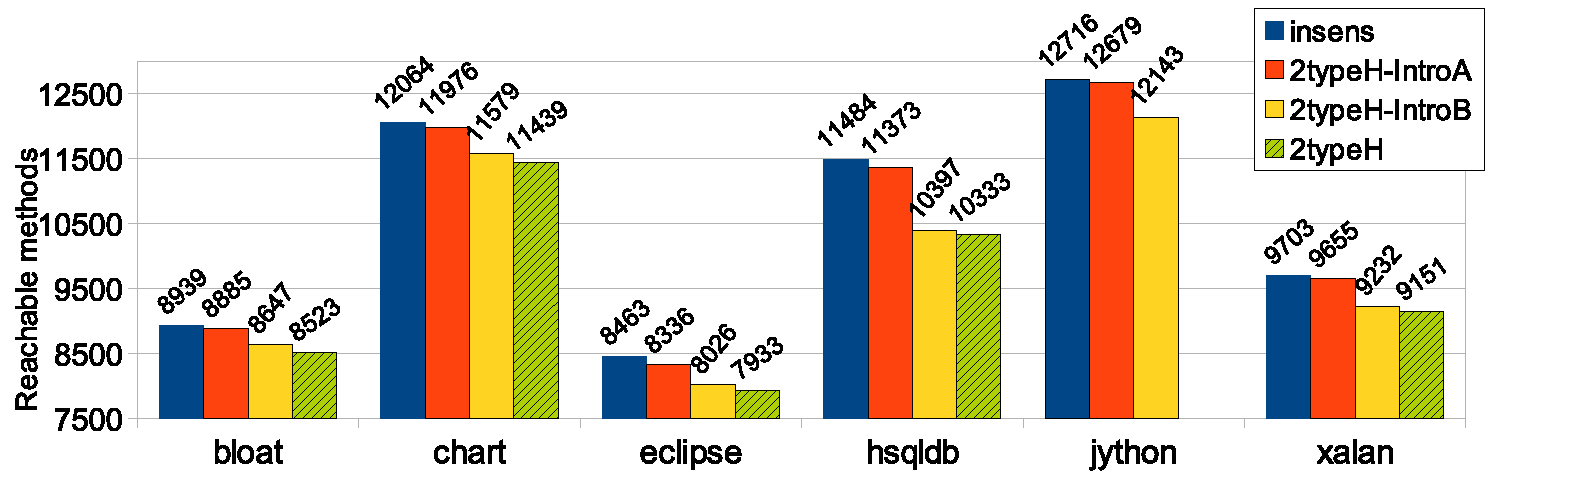
\includegraphics[scale=0.54]{assets/introspective/2typeHmeths.pdf} \\
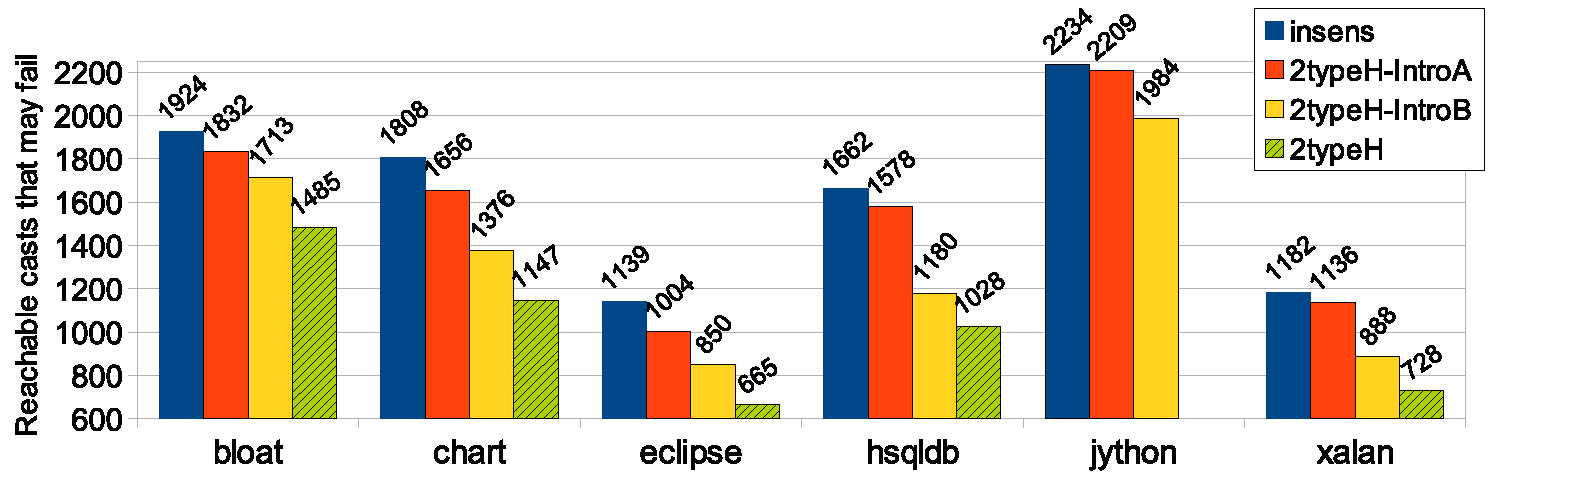
\includegraphics[scale=0.54]{assets/introspective/2typeHcasts.pdf}
\end{center}
\vspace{-0.65cm}
\caption{Performance and precision (3 separate metrics: calls that
  cannot be devirtualized, reachable methods, casts that cannot be
  eliminated) for introspective context-sensitive
 variants of a 2typeH analysis, compared with baselines (2typeH and insensitive).}
\label{2typeH-chart}
\end{figure*}

\begin{figure*}[tbp]
\begin{center}
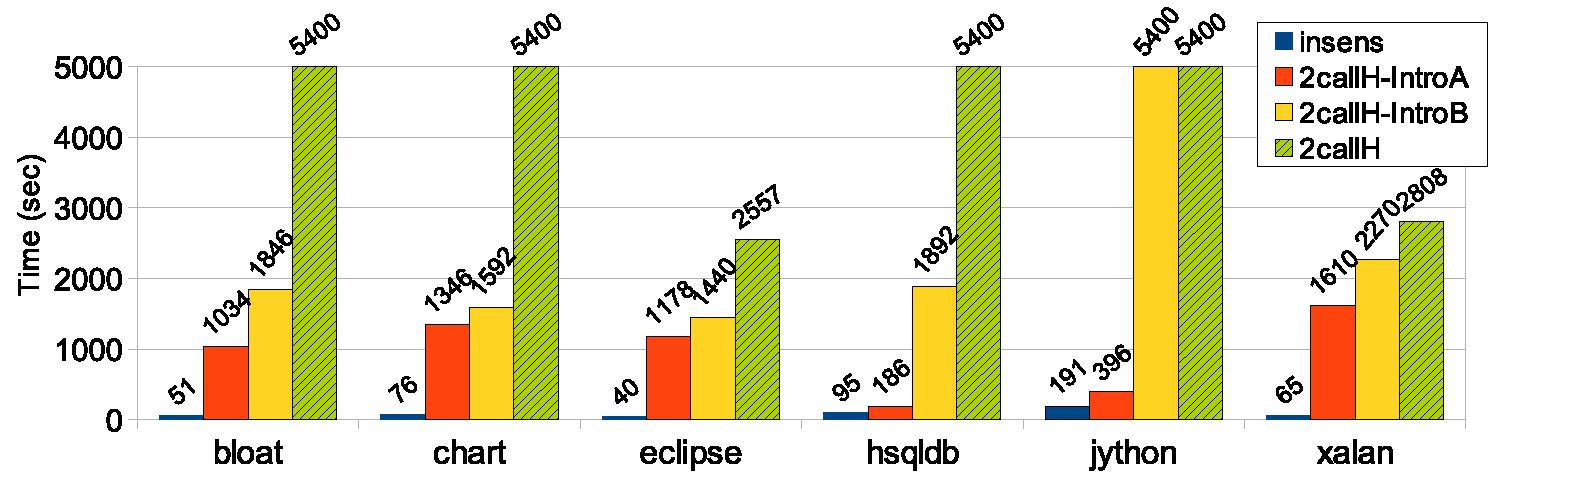
\includegraphics[scale=0.54]{assets/introspective/2callHtime.pdf} \\
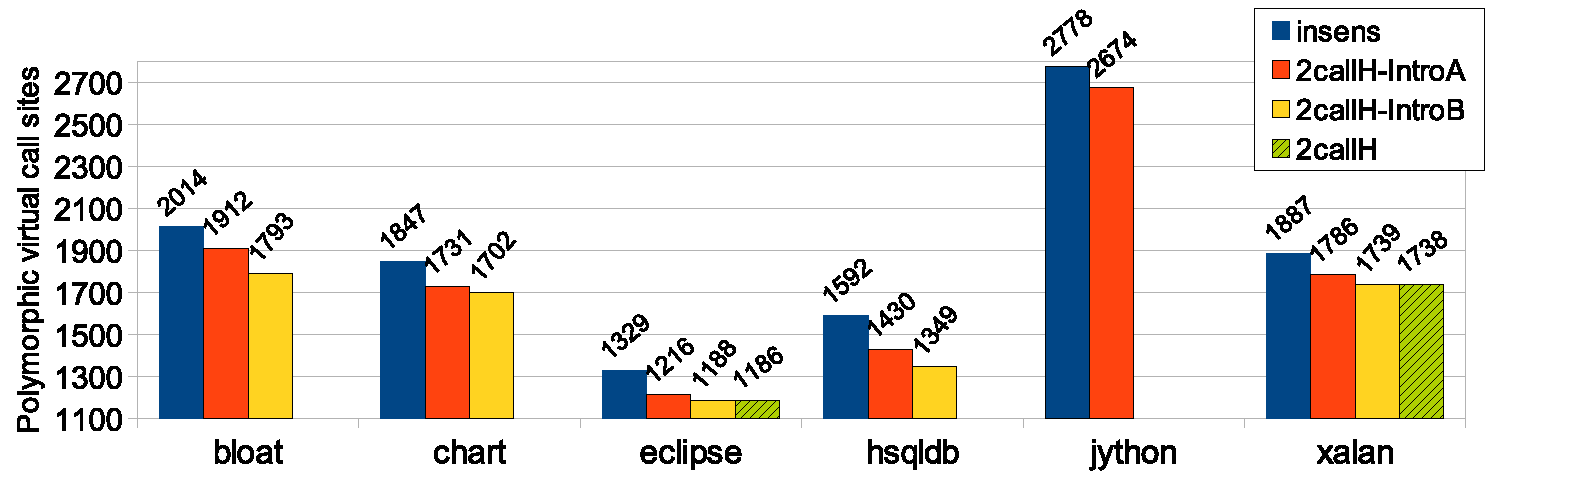
\includegraphics[scale=0.54]{assets/introspective/2callHvcalls.pdf} \\
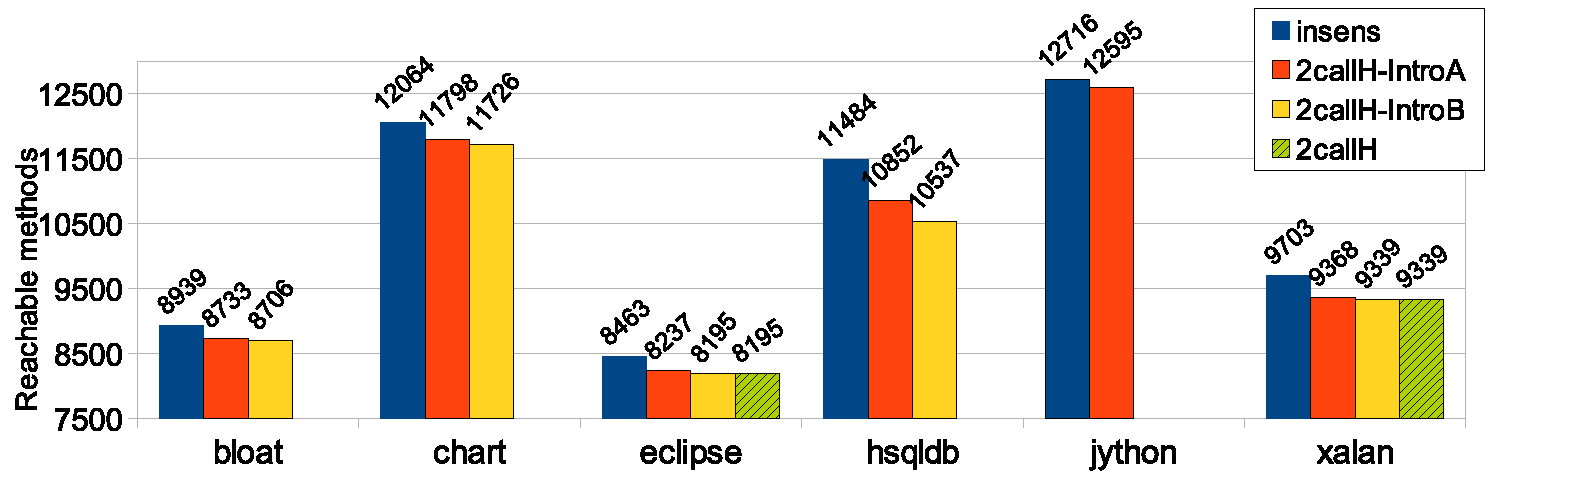
\includegraphics[scale=0.54]{assets/introspective/2callHmeths.pdf} \\
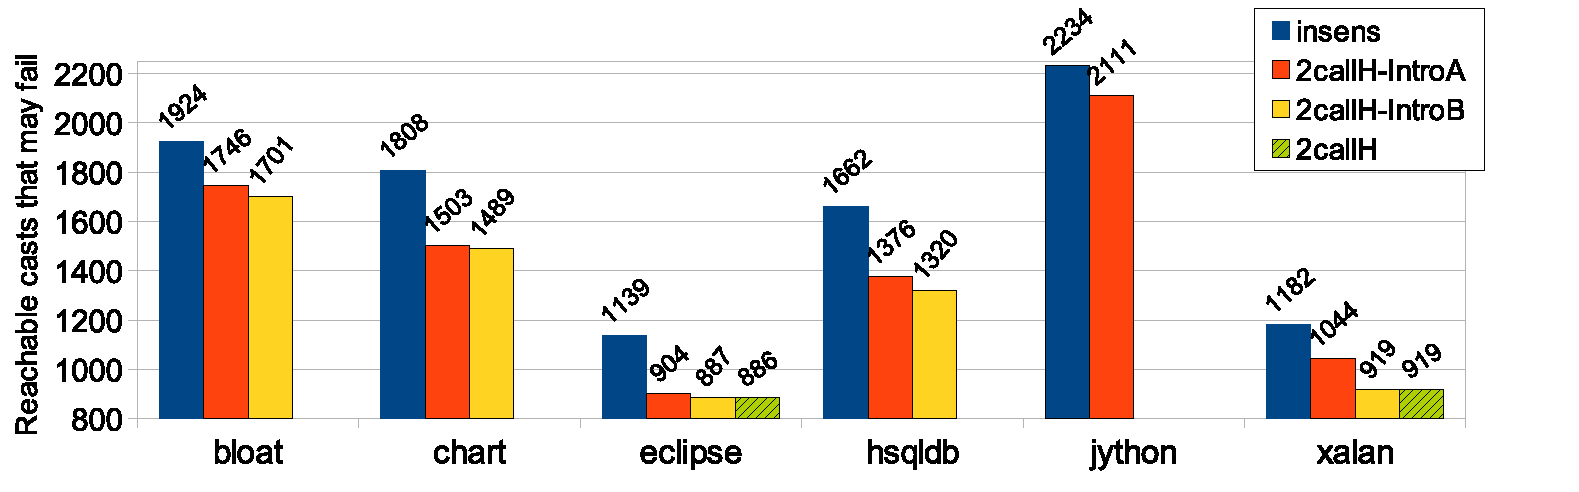
\includegraphics[scale=0.54]{assets/introspective/2callHcasts.pdf}
\vspace{-0.65cm}
\end{center}
\caption{Performance and precision (3 separate metrics: calls that
  cannot be devirtualized, reachable methods, casts that cannot be
  eliminated) for introspective context-sensitive
 variants of a 2callH analysis, compared with baselines (2callH and insensitive).}
\label{2callH-chart}
\end{figure*}

The results of our experiments are shown in Figures~\ref{2objH-chart},
\ref{2typeH-chart}, and \ref{2callH-chart}. We evaluate two variants
of introspective context-sensitivity corresponding to \emph{Heuristic
  A} and \emph{Heuristic B} from Section~\ref{heuristics}. We test the
three main flavors of context-sensitivity: object-sensitivity
\cite{Milanova:2002:POS:566172.566174,1044835}, call-site sensitivity
\cite{Sharir:Interprocedural,Shivers:1991:diss}, and
type-sensitivity~\cite{pointsto-popl11}. The three flavors have very
different profiles of practical use and scalability, as detailed next.

\paragraph{Object-sensitivity.}
Deep-context object-sensitive analyses are the most precise in
practice, but do not always scale well. Starting from a
2-object-sensitive analysis with a (1-)context-sensitive heap (2objH),
we define our two introspective versions (2objH-IntroA and
2objH-IntroB for \emph{Heuristic A} and \emph{Heuristic B},
resp.). Figure~\ref{2objH-chart} plots first the execution time and
then three precision metrics for all analyses.
%The combination of all three metrics gives a good projection of
%precision, although for different client analyses precision could
%vary.
In all cases \emph{lower is better}. There is no real ``metric'' for
precision, since each client may have unique needs, but our three
metrics together should yield a reasonable projection of
precision. Note that since there is no ``ground truth'' for the ideal
value of precision metrics, their chart scales are arbitrary (and
differences are not as visually pronounced as could be because of
plotting multiple benchmarks on a single chart) but the
insensitive/2objH analyses serve as upper/lower reference markers in
practice. We use a 90min timeout. The jython and hsqldb benchmarks did
not terminate for 2objH, and jython did not terminate for 2objH-IntroB
either. We indicate non-termination with full bars in the top (time)
chart and the absence of bars in the bottom three (precision) charts.

As can be seen, the two introspective variants scale much better than
the full 2objH analysis. Indeed, IntroA scales to all benchmarks,
while showing significant precision gains over an insensitive
analysis. IntroB is even more precise: it covers \emph{more than
  two-thirds} of the precision advantage of 2objH over an insensitive
analysis for most benchmarks and precision metrics, while scaling
significantly better.



\paragraph{Type-sensitivity.}
Type-sensitivity is designed with the explicit purpose of providing
more scalability than object-sensitivity but in a very different
manner: instead of avoiding high context depths, type-sensitivity
makes each context element coarser. Thus it is doubly interesting to
see if introspection can add benefit to type-sensitive analyses.
Type-sensitivity is not immune to the pathologies of
object-sensitivity: for instance, in our benchmark set it does not
scale to jython. 

Figure~\ref{2typeH-chart} shows our results, plotting variants of a
2-type-sensitive analysis with a (1-)context-sensitive heap (2typeH),
and following the same conventions as earlier. (The insensitive
baseline is inherited and not re-run.) As can be seen, the IntroB
version scales to all programs while typically maintaining very good
precision---often close to the full 2typeH. The IntroA version has the
desirable feature of near-perfect scalability: its maximum runtime for
\emph{any} benchmark is 360sec. At the same time it exhibits precision
gains compared to a context-insensitive analysis, although these are
noticeably lower than the precision gains of IntroB.

\paragraph{Call-site sensitivity.}
Call-site sensitivity is the traditional flavor of
context-sensitivity---a virtual synonym for the term. In practice,
call-site sensitivity is quite good for some analysis clients but
almost never scalable at context depths greater than 1. 

As Figure~\ref{2callH-chart} shows, introspective context-sensitivity
performs remarkably well when applied to a 2-call-site-sensitive
analysis with a (1-)context-sensitive heap (2callH). The base 2callH
analysis does not terminate for 4-out-of-6 of our benchmarks, while
introspective analyses terminate either for all (IntroA) or for nearly
all (5-out-of-6 for IntroB).  Furthermore, IntroB seems to achieve the
full precision of 2callH for the two benchmarks for which the latter
yields results, and for all different metrics! Combined with the
across-the-board scalability gains shown in the timing chart, this
confirms the effectiveness of introspection for tuning out extreme
analysis costs.  IntroA is not far behind in precision, obtaining more
than two-thirds of the precision gains of IntroB for most metrics and
benchmarks.


\paragraph{Discussion.}

The above timings of introspective context-sensitivity do not include
the cost of first running a context-insensitive analysis, and other
timing overheads (relatively constant at about 100sec) related to
computing the objects and sites to refine and re-running an analysis
(our current implementation saves the first-run database and
re-generates it from scratch). We did not include these numbers in the
timings in order to keep the presentation simpler but also because (a)
our emphasis is on scalability and not on small-scale speed gains---we
consider small differences in timings, e.g., in the chart and eclipse
benchmarks of Figure~\ref{2objH-chart}, to be negligible for our
purposes; and (b) these constant overheads can be factored out---e.g.,
with minor engineering we could have incurred them only once per
benchmark and not once per run of every introspective analysis
variation.

% but on arguing that introspective analyses are
%qualitatively more scalable: they give a way to go where other
%analyses cannot.

Based on our experimental results, introspective context-sensitivity
achieves its goal: it offers a knob for users to select
points in the scalability/precision spectrum. The tradeoffs of cost
and precision exhibited by \emph{Heuristic A} and \emph{Heuristic B}
are illustrative. Not only do these heuristics yield different options
(more precision vs. more scalability) but they are also very
consistent in their tradeoff, throughout multiple benchmarks and
analysis flavors.

Finally note that we used identical introspection heuristics
(\emph{Heuristic A} and \emph{Heuristic B}) with the same constants
(see Section~\ref{heuristics}) for all three context-sensitivity
flavors and for all benchmarks. This suggests that there are
significant opportunities for further tuning: different heuristics can
be used, the constants can be optimized, the constants or the heuristics
can be adapted per-benchmark or per-context flavor. However, the goal
of our experiments is not to squeeze out a few percentage points of
speedup but to show that the simple idea of introspective
context-sensitivity can easily offer very useful tradeoffs in
scalability and precision.


\section{Related Work}
\label{sec:related}

The effort to tune the context-sensitivity of an analysis is pervasive
in the literature. Nevertheless, most approaches fundamentally differ
from ours, either by trying to vary context-sensitivity based on
syntactic properties or by trying to focus on only a part of the program
that matters for answering a given query.
In contrast, we attack the context-sensitive scalability problem 
head-on, in the all-points points-to analysis setting, with context
used all over the program and library.

Typical scalable points-to analysis frameworks such as
Wala~\cite{www:wala} and Doop~\cite{BS-OOPSLA09} employ a multitude of
low-level heuristics for tuning the precision and scalability of an
analysis. These include using extra context for collection classes,
using a heap context for arrays in an analysis without a
context-sensitive heap, allocating strings or exceptions
context-insensitively, treating library factory methods with deeper
context, etc. Such heuristics are typically user-selected and
prominent in the documentation of the respective frameworks, and have
also appeared in the literature (e.g.,
\cite{Tripp:2009:TET:1542476.1542486,exceptions-cc13}).  However, all
such approaches are mere hard-wired heuristics and do not address the
major scalability problem that our approach aims to solve. The
scalability issues identified in earlier literature and discussed
throughout this paper are present after all such heuristics have been
employed.
% These
%heuristics are already implemented in the baseline framework that we
%use for our analysis. 

A more general approach is \emph{hybrid} context-sensitivity, which
consists of treating virtual and static method calls differently
\cite{hybrid-pldi13}. Such a hybrid analysis attempts to emulate
call-site sensitivity for static method calls and object-sensitivity
for dynamic calls. The approach becomes interesting when context is
deep (e.g., how are context elements merged when a dynamic call is
made inside a static call?). Nevertheless, the hybrid
context-sensitivity approach does not change the essence of the
problem we are trying to solve. For hard-to-analyze applications,
hybrid context-sensitive algorithms are equally unscalable as their
component algorithms. For the purposes of our experimental study,
which only tests the scalability of heavyweight benchmarks, hybrid
context-sensitivity is virtually indistinguishable from object-
sensitivity.

More interesting applications of selective context-sensitivity have
been explored in the context of \emph{demand-driven} pointer analysis.
A demand-driven evaluation strategy reduces the cost of an analysis by
computing only those results that are necessary for a client program
analysis~\cite{1094817,1134027,1328464,378802}. This is a useful
approach for client analyses that focus on specific locations in a
program, but if the client needs results from the entire program, then
demand-driven analysis is typically slower than an exhaustive
analysis.

In the demand-driven space, refinement-based analyses have been used
primarily in the work of Sridharan and Bod\'{\i}k~\cite{1134027} and
of Liang and Naik~\cite{Liang:2011:SAR:1993498.1993567}.  Sridharan
and Bod\'{\i}k~\cite{1134027} introduce refinement-based analysis as a
way to adaptively increase the precision characteristics of an
existing analysis algorithm when a client analysis is not satisfied
with the result. The approach allows turning on field-sensitivity, as
well as higher call-site sensitivity for an analysis algorithm. Yet,
unlike ours, it is not a general approach that can apply to any kind
of context and a large number of different algorithms.  Liang and
Naik's ``pruning'' approach \cite{Liang:2011:SAR:1993498.1993567}
consists of first computing a coarse over-approximation of the
points-to information, while keeping the provenance of this
derivation, i.e., recording which input facts have affected each part
of the output. The input program is then pruned so that parts that did
not affect the interesting points of the output are eliminated. Then a
highly context-sensitive precise analysis is run, in order to
establish the desired property. This approach is similar to
introspective context-sensitivity in that the analysis is run twice
and a separate query over the first-run result determines the second
run's characteristics.  Nevertheless, our approach requires no
provenance computation (which is unlikely to scale for an all-points
analysis) and works even when we want answers for the entire
program---i.e., when pruning is not possible.

Both of the above demand-driven approaches can be viewed as
complements of our introspective context-sensitivity. In the
demand-driven world, it is possible to estimate the \emph{benefit}
that a more precise analysis may yield: either the client is happy
with the current level of precision (which implies there is no further
benefit to be obtained) or it is not, in which case more precision
should be added. In our all-points pointer analysis problem we have no
such information. This motivates our \emph{cost}-based heuristics,
which attempt to estimate ``what can go wrong'' when more precision
gets added, as opposed to ``what can be gained'', as in demand-driven
techniques.

\section{Conclusions}

We introduced introspective context-sensitivity: an approach to making
context-sensitive analyses scale. The approach consists of defining an
analysis with two separate kinds of context. Each program element is
analyzed with one kind, selected based on external input. Then, by
first running an inexpensive context-insensitive analysis, we can
identify program elements that should be treated with a more precise
context and others that should be treated less precisely to avoid an
explosion in complexity. Our technique applies to any kind of context
abstraction and yields scalability \emph{\`{a} la carte}: the user can
select a scalability profile and achieve it for a price in
precision. As shown in our experiments, this price is not too
steep. The precision loss of introspective context-sensitivity can be
minuscule (as is for call-site-sensitive analyses), while the
scalability gain is substantial. 

We believe that introspective context-sensitivity is a big step
forward in pointer analysis. It is not just an effective technique,
but an effective technique that addresses the major current pain point
in practical applications of points-to analyses.

% \begin{comment}

% \acks We gratefully acknowledge funding by the European Union under a
% Marie Curie International Reintegration Grant and a European Research
% Council Starting/Consolidator grant; and by the Greek Secretariat for
% Research and Technology under an Excellence (Aristeia) award. We thank
% the anonymous reviewers, who offered several valuable suggestions, and
% LogicBlox Inc. for providing our Datalog engine, as well as
% technical and material support.

% \end{comment}